% Figure 1.2 (Session 1): the Hubbard chain and the spinless chain side by side.
% The image is rendered by figures/blender/s1_2_two_interactions.py; the coordinates of the labels
% come from figures/blender/out/two_interactions_anchors.tex. Compile with:
%   pdflatex two_interactions.tex ; result moves to ../classical_magnetism/two_interactions.pdf
\documentclass[11pt,tikz,border=0pt]{standalone}
\usepackage{amsmath,amssymb,graphicx}
\usepackage{xcolor}
\definecolor{coursedark}{HTML}{1B2A4A}
\definecolor{costamber}{HTML}{B8620A}
\newlength{\figw}\setlength{\figw}{16.19cm}   % the text width of the notes (letter, 2.7 cm margins), so labels print at size

\begin{document}
\begin{tikzpicture}[lbl/.style={font=\small, text=coursedark}]
  \node[anchor=south west, inner sep=0pt] at (0,0)
    {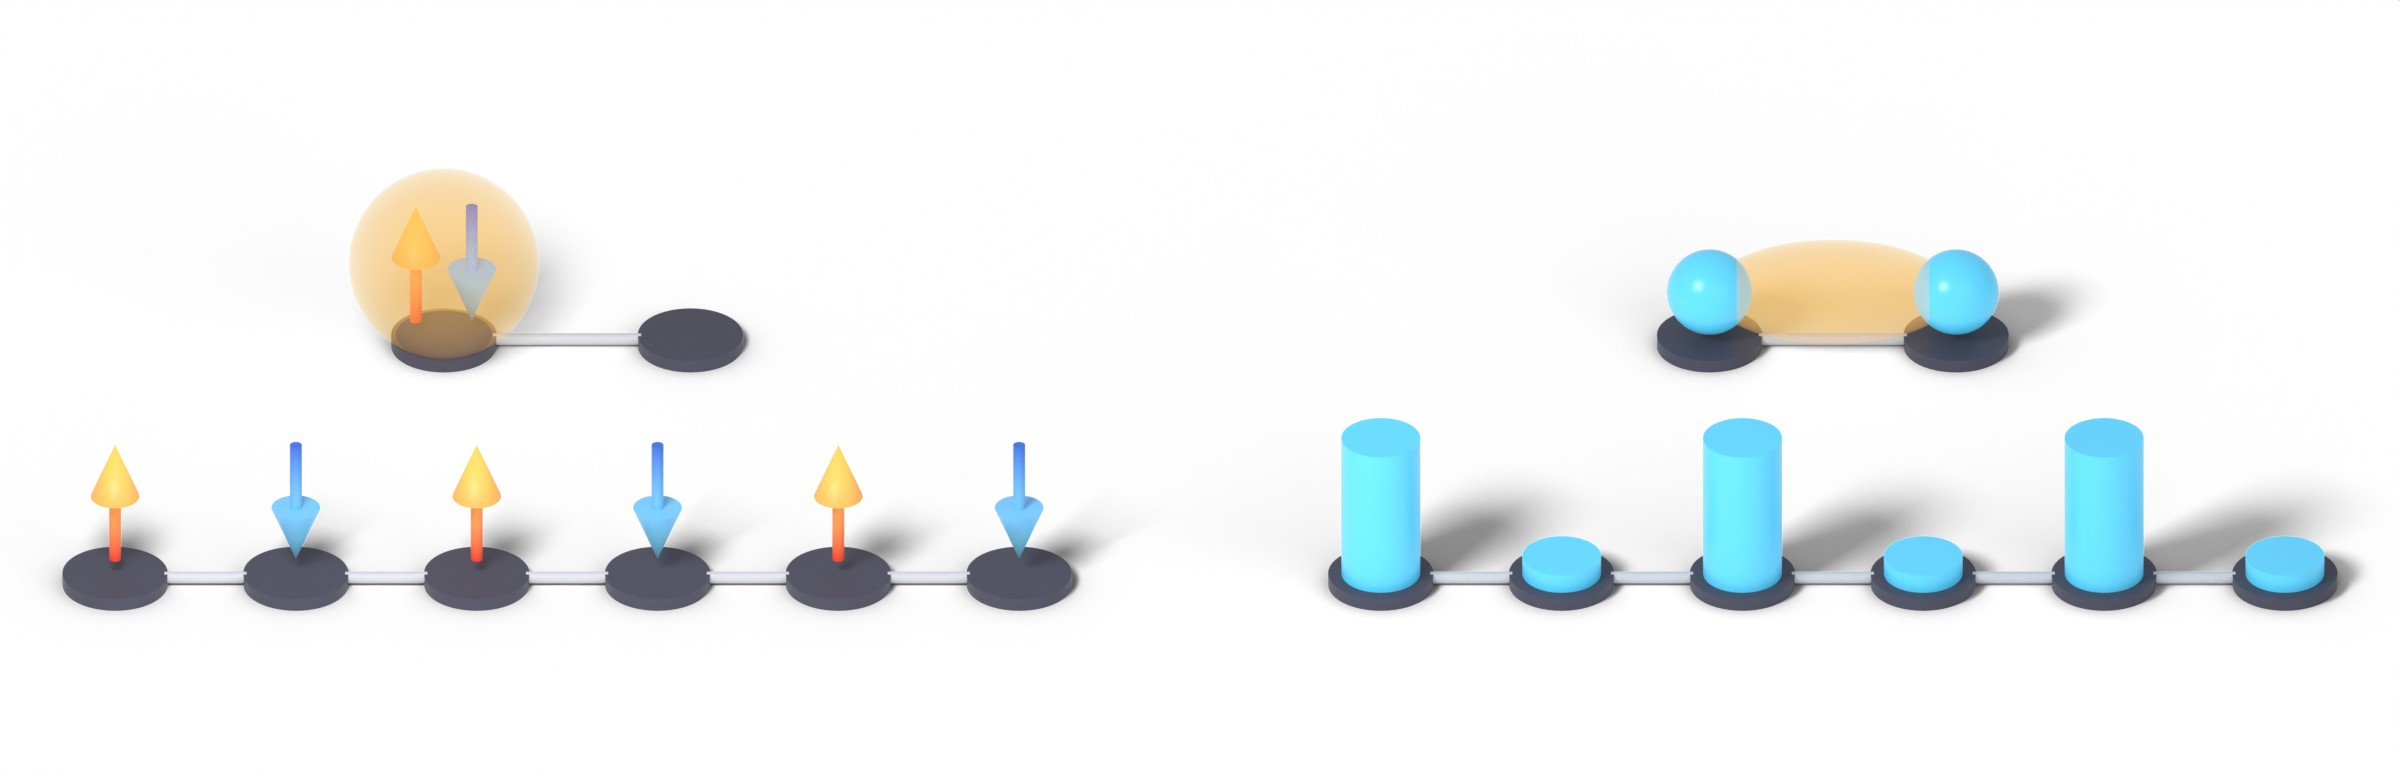
\includegraphics[width=\figw]{../blender/out/two_interactions.jpg}};
  %% written by figlib.py; x and y in units of the image width
\coordinate (U) at (0.2226\figw,0.2423\figw);
\coordinate (a) at (0.0171\figw,0.2910\figw);
\coordinate (chainA) at (0.2363\figw,0.0481\figw);
\coordinate (V) at (0.7637\figw,0.2394\figw);
\coordinate (b) at (0.5445\figw,0.2910\figw);
\coordinate (chainB) at (0.7637\figw,0.0481\figw);

  \node[lbl, font=\normalsize, anchor=west] at (a) {(a)};
  \node[lbl, font=\normalsize, anchor=west] at (b) {(b)};
  \node[lbl, text=costamber, anchor=west] at (U) {$U\,n_{i\uparrow}n_{i\downarrow}$};
  \node[lbl, text=costamber, anchor=south] at (V) {$V\,n_i n_{i+1}$};
  \node[lbl, anchor=north] at (chainA) {magnetic order};
  \node[lbl, anchor=north] at (chainB) {charge density wave};
\end{tikzpicture}
\end{document}
